\chapter{Resultados}

En este capítulo se van a mostrar resultados obtenidos con las siguientes funcionalidades implementadas: Filtrado, segmentación y documentación.

Para realizar las pruebas se han utilizado la esculturas de Inmaculada Concepción y San Juan Evangelista (Figura \ref{fig:resultados/esculturas}), ambas patrimonio de la Universidad de Granada y cuyos datos DICOM han sido proporcionados por el proyecto de Portal Virtual de Patrimonio de las Universidades Andaluzas, coordinado por la Universidad de Granada.

\begin{figure}[H]
	\centering
	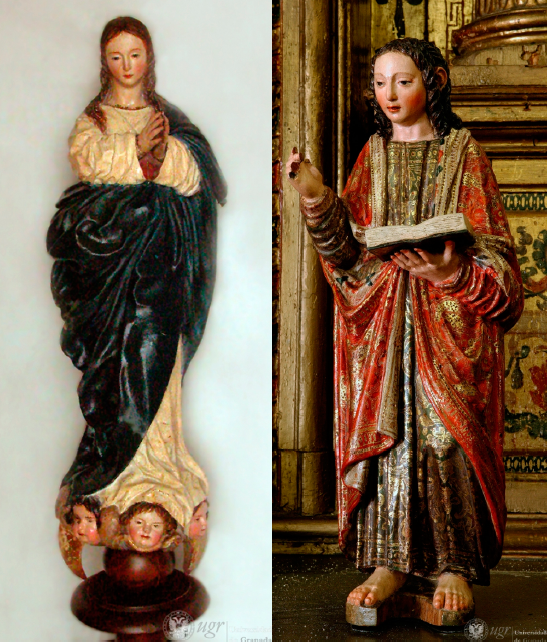
\includegraphics[width=7cm]{imagenes/resultados/esculturas}
	\caption{Esculturas utilizadas para realizar las pruebas. Inmaculada Concepción (izquierda) y San Juan Evangelista (derecha)}
	\label{fig:resultados/esculturas}
\end{figure}

\section{Filtrado}

Se implementaron los filtros de reducción de ruido \textit{gaussiano}, media y mediana dando la posibilidad al usuario a elegir ciertos parámetros.

Para probar estos filtros se ha utilizado la escultura de San Juan Evangelista que es la que más ruido presentaba.

\subsection{Filtro \textit{gaussiano}}

El filtro \textit{gaussiano} es uno de los filtros de suavizado más utilizados. A continuación se va a mostrar los resultados obtenidos con éste para 1, 2 y 3 repeticiones (Figura \ref{fig:resultados/filtrado/gaussiano}).

\begin{figure}[H]
	\centering
	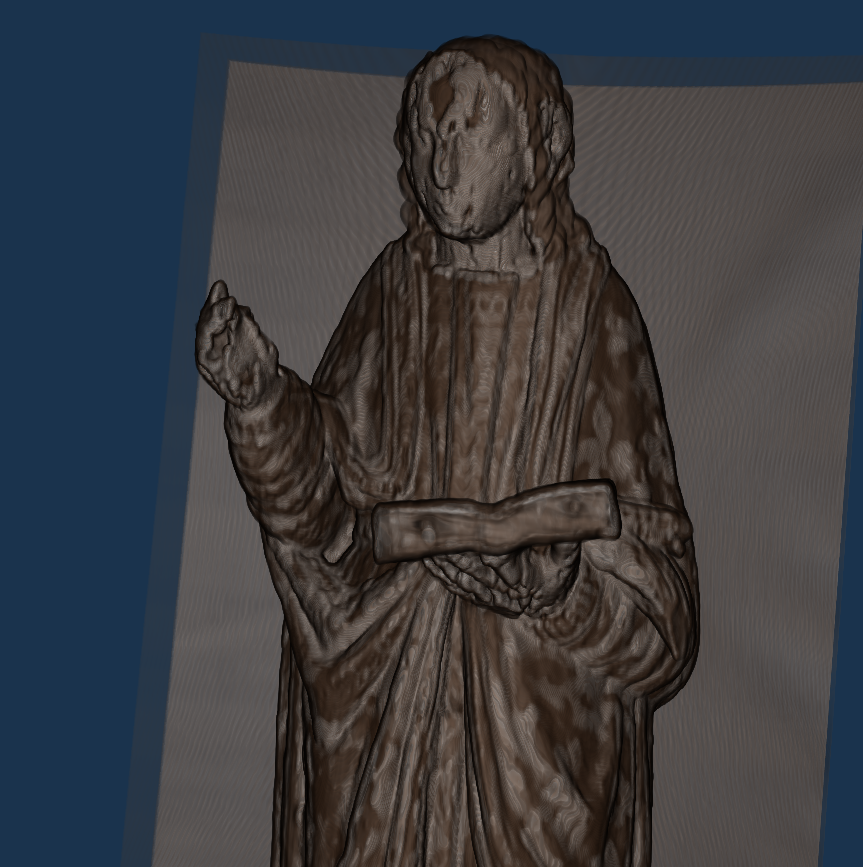
\includegraphics[width=6cm]{imagenes/resultados/filtrado/original}
	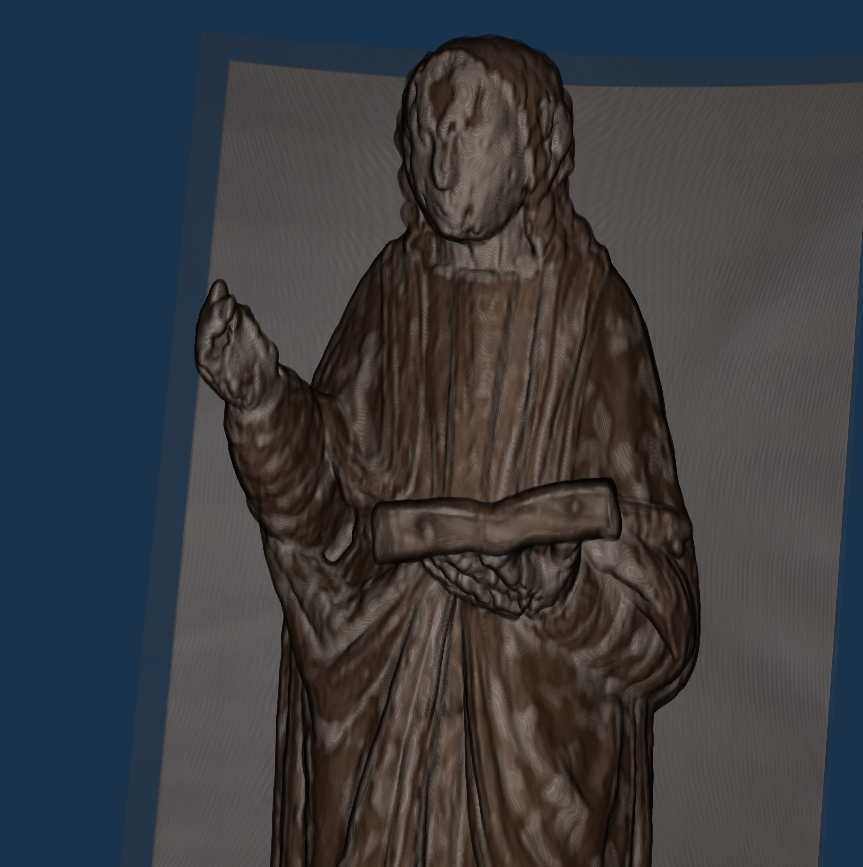
\includegraphics[width=6cm]{imagenes/resultados/filtrado/gaussiano-1}
	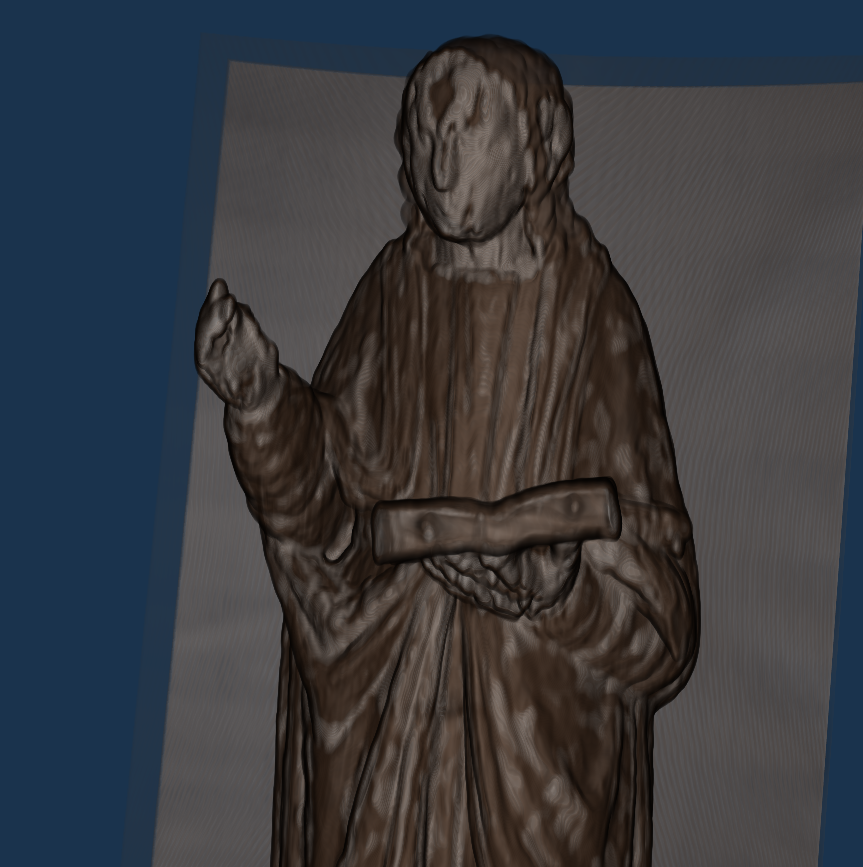
\includegraphics[width=6cm]{imagenes/resultados/filtrado/gaussiano-2}
	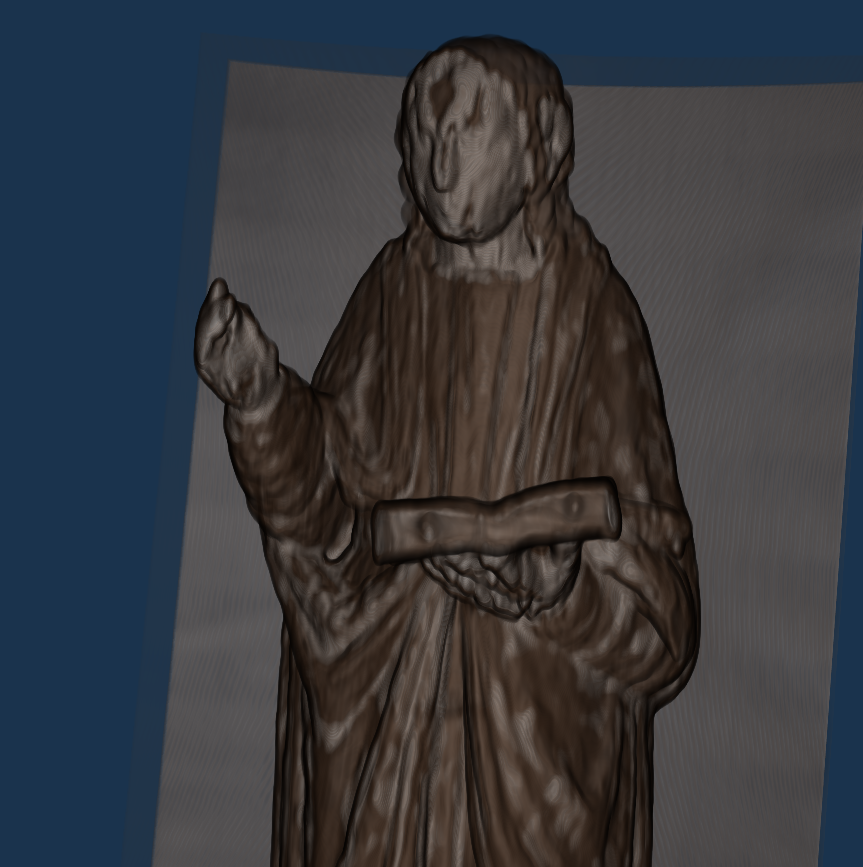
\includegraphics[width=6cm]{imagenes/resultados/filtrado/gaussiano-3}
	\caption{De izquierda a derecha y arriba a abajo: figura original y aplicando el filtro \textit{gaussiano} con 1, 2 y 3 repeticiones}
	\label{fig:resultados/filtrado/gaussiano}
\end{figure}

Se puede observar como apenas hay diferencia entre la original y la que se le ha aplicado el filtro con una sola repetición.

Con la que mejor resultado se obtiene es con la que se le aplica 2 repeticiones, porque con 3 ya empieza a suavizarse de más.

\subsection{Filtro media}

El filtro media es un filtro de suavizado bastante agresivo que usa una convolución y donde el único parámetro que se puede utilizar es el tamaño del vecindario para la convolución. A continuación se va a mostrar los resultados obtenidos con éste para vecindarios de 3x3, 5x5 y 7x7 (Figura \ref{fig:resultados/filtrado/media}).

\begin{figure}[H]
	\centering
	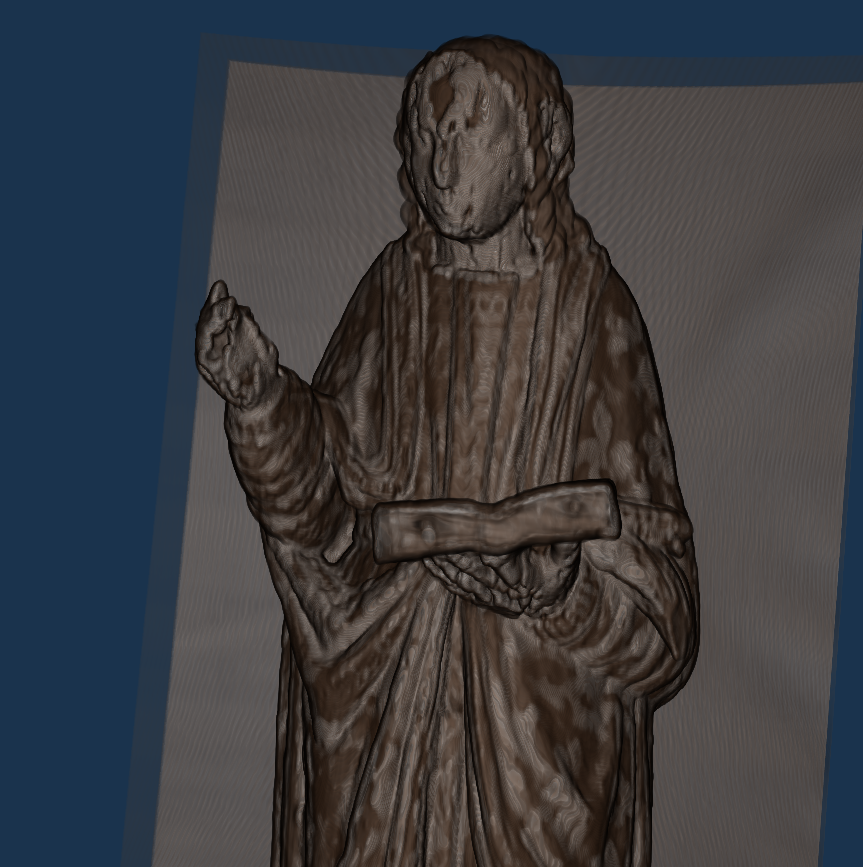
\includegraphics[width=6cm]{imagenes/resultados/filtrado/original}
	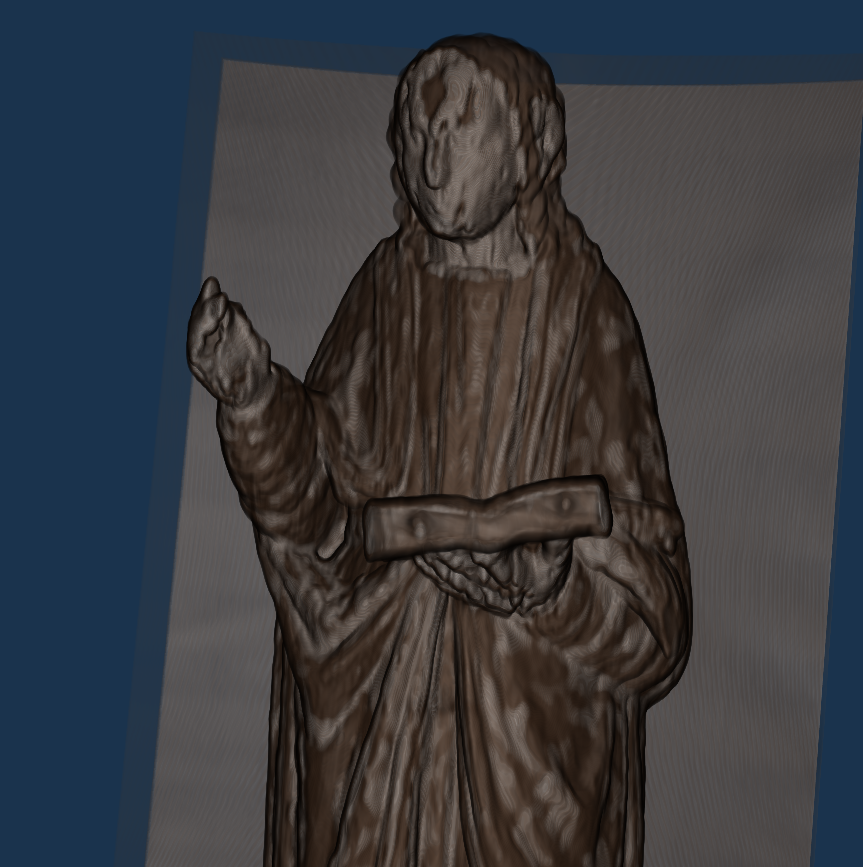
\includegraphics[width=6cm]{imagenes/resultados/filtrado/media-3}
	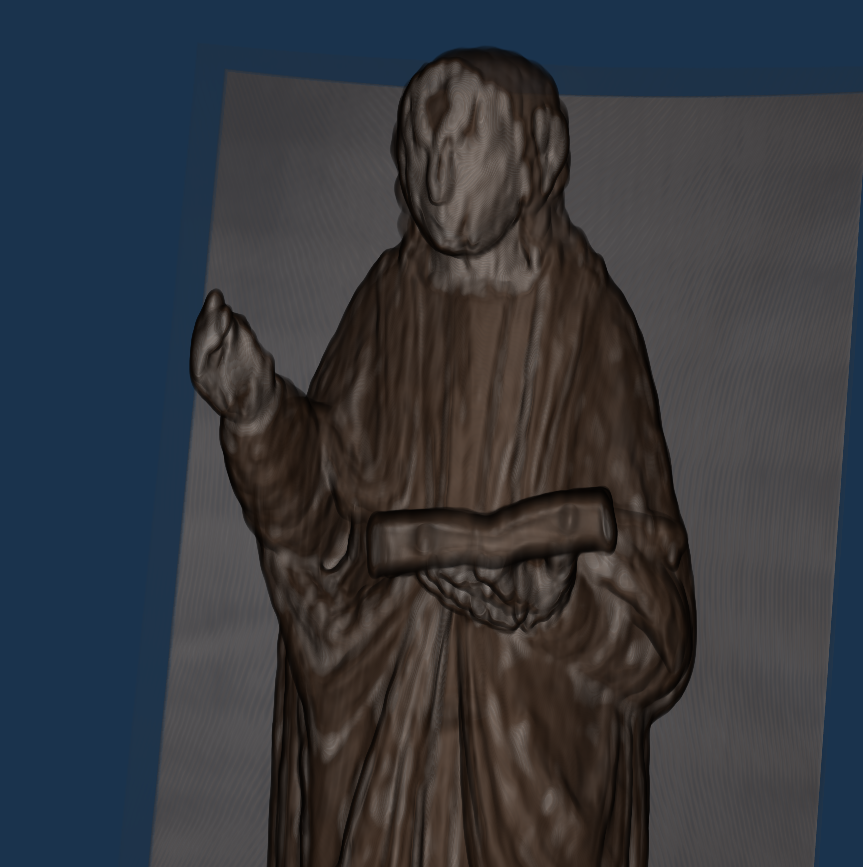
\includegraphics[width=6cm]{imagenes/resultados/filtrado/media-5}
	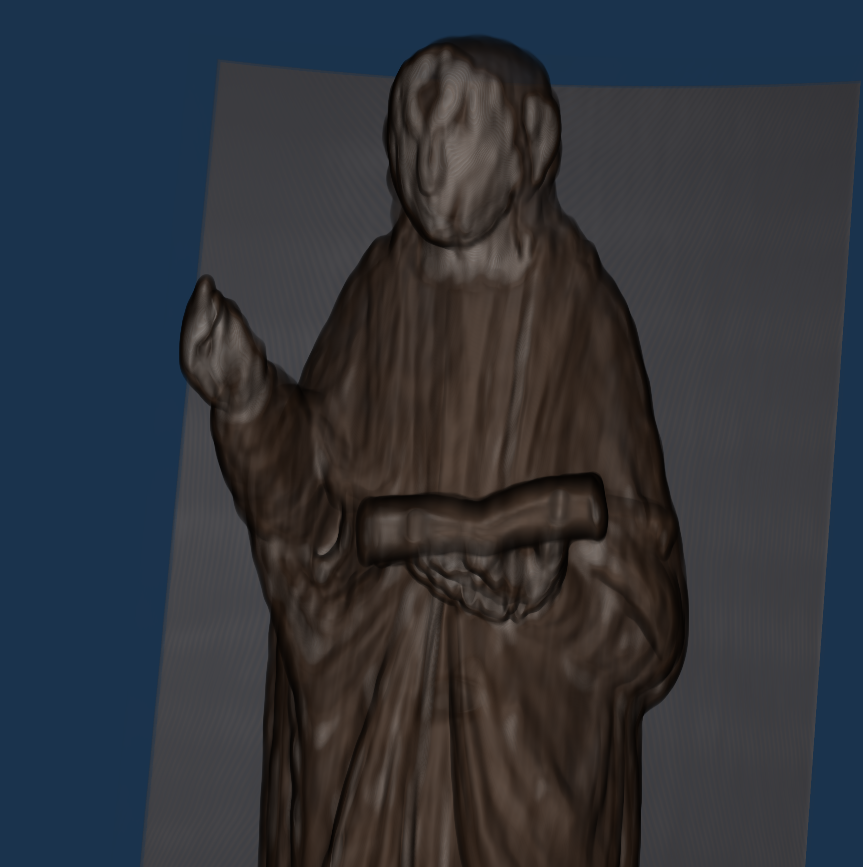
\includegraphics[width=6cm]{imagenes/resultados/filtrado/media-7}
	\caption{De izquierda a derecha y arriba a abajo: figura original y aplicando el filtro media con vecindarios de 3x3, 5x5 y 7x7}
	\label{fig:resultados/filtrado/media}
\end{figure}

Se puede ver como este filtro es bastante más agresivo que el \textit{gaussiano} y se suaviza de más. Por tanto, habría que utilizarlo para imágenes con mucho más ruido.

\subsection{Filtro mediana}

El filtro mediana se utiliza para reducir el ruido de tipo \textit{salt-and-pepper}. Nuestras imágenes no sufren de este tipo de ruido. No obstante se ha probado el filtro con vecindarios de 3x3, 5x5 y 7x7 (Figura \ref{fig:resultados/filtrado/mediana}).

\begin{figure}[H]
	\centering
	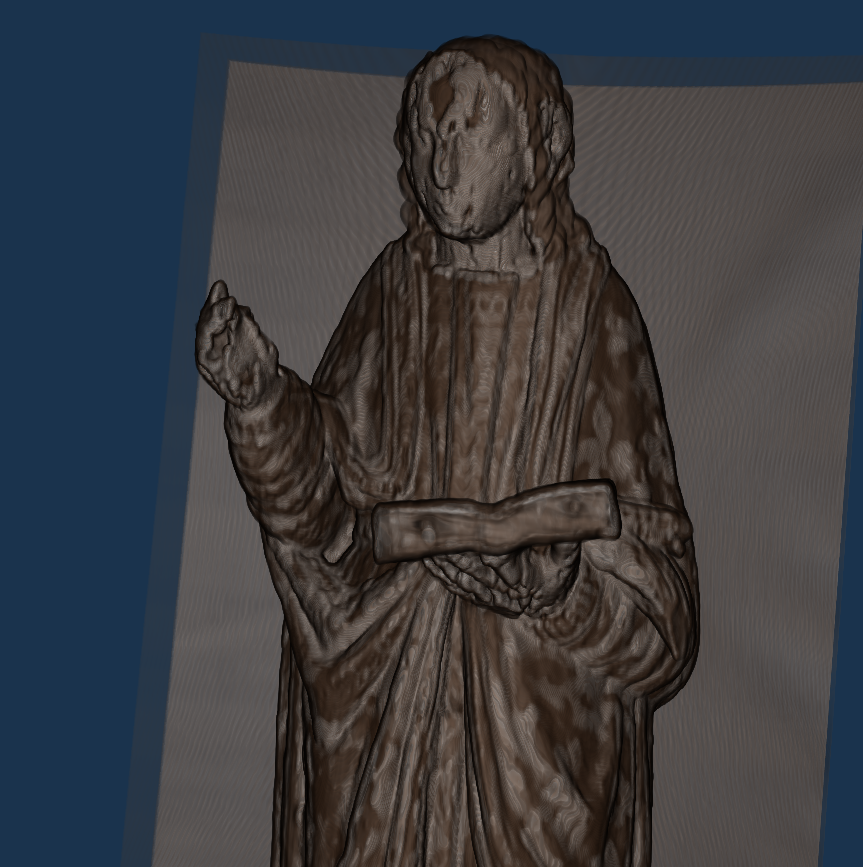
\includegraphics[width=6cm]{imagenes/resultados/filtrado/original}
	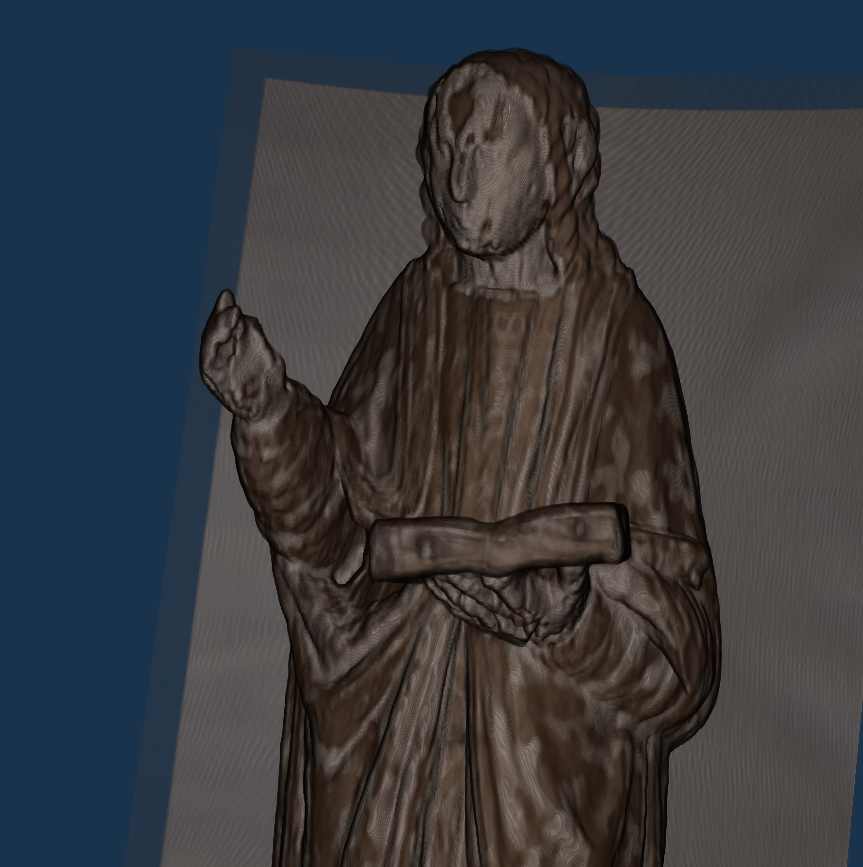
\includegraphics[width=6cm]{imagenes/resultados/filtrado/mediana-3}
	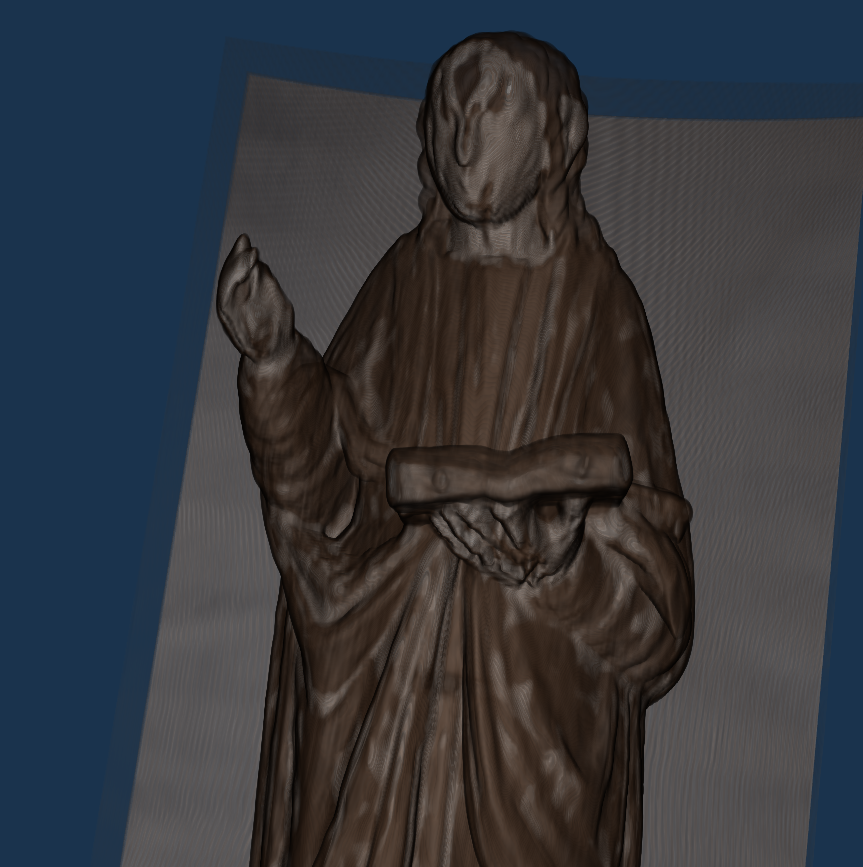
\includegraphics[width=6cm]{imagenes/resultados/filtrado/mediana-5}
	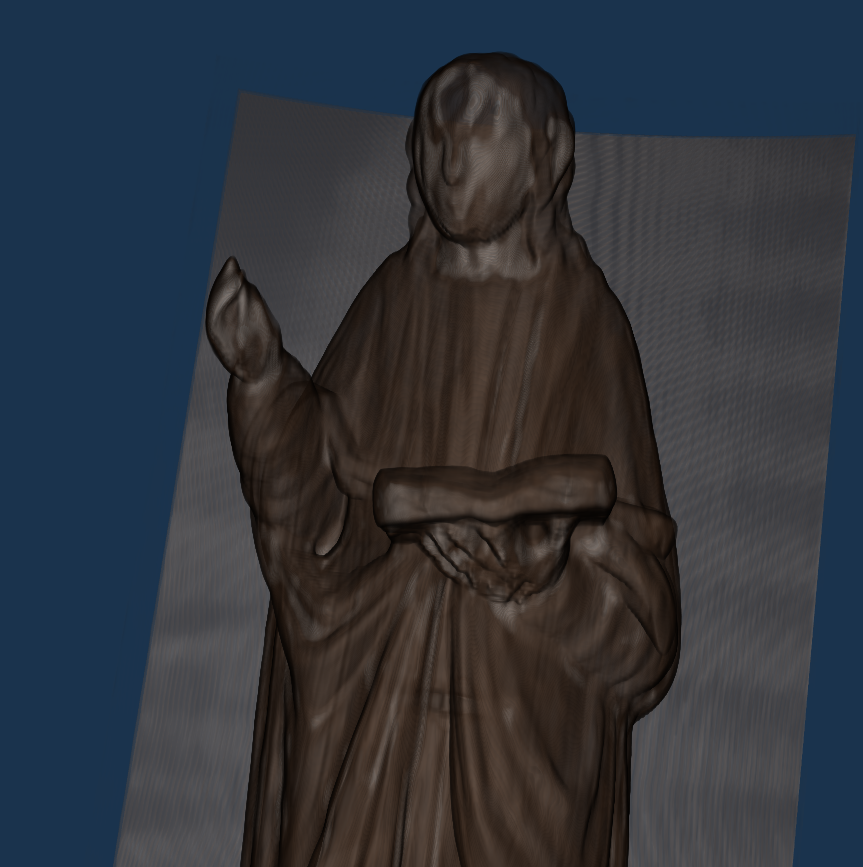
\includegraphics[width=6cm]{imagenes/resultados/filtrado/mediana-7}
	\caption{De izquierda a derecha y arriba a abajo: figura original y aplicando el filtro mediana con vecindarios de 3x3, 5x5 y 7x7}
	\label{fig:resultados/filtrado/mediana}
\end{figure}

Los resultados con este filtro son incluso más agresivos que los obtenidos con el de media. Pero es lógico al ser un filtro creado para reducir un tipo de ruido que no presentan nuestras imágenes.

\section{Segmentación}

Se ha probado el método de segmentación propuesto para separar las piezas del embón de ambas esculturas.

\subsection{Inmaculada Concepción}

En la Inmaculada Concepción hay dos piezas principales en el embón a derecha e izquierda que se puede contemplar muy bien en cualquier corte axial desde la altura del pecho hasta abajo. Por tanto se podría usar como semilla cualquiera de estos cortes pues seguramente encuentre la línea que separa ambas partes entre las líneas rectas más grandes encontradas en este corte.

Se ha utilizado uno de estos cortes y se ha encontrado fácilmente esta línea (Figura \ref{fig:resultados/segmentacion/inmaculada-concepcion/seleccion-linea}).

\begin{figure}[H]
	\centering
	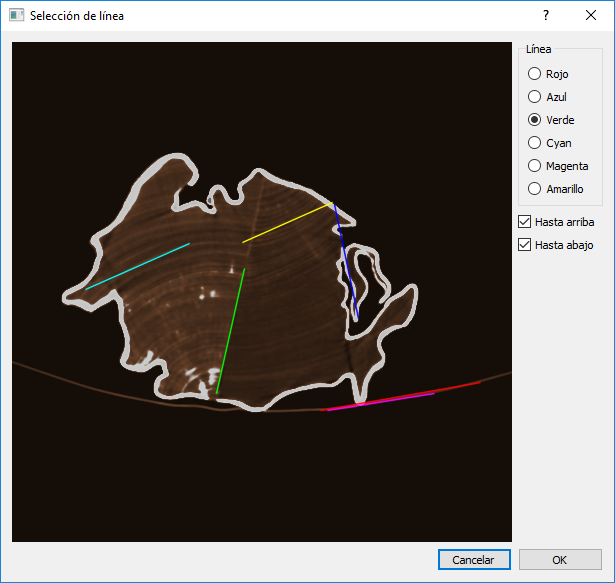
\includegraphics[width=12cm]{imagenes/resultados/segmentacion/inmaculada-concepcion/seleccion-linea}
	\caption{Líneas encontradas en un corte a la altura de la cintura donde se ve la línea (verde) que separa las dos piezas del embón}
	\label{fig:resultados/segmentacion/inmaculada-concepcion/seleccion-linea}
\end{figure}

Esta línea divide perfectamente en dos la figura obteniendo los resultados de a continuación (Figuras \ref{fig:resultados/segmentacion/inmaculada-concepcion/dcha} y \ref{fig:resultados/segmentacion/inmaculada-concepcion/dcha}).

\begin{figure}[H]
	\centering
	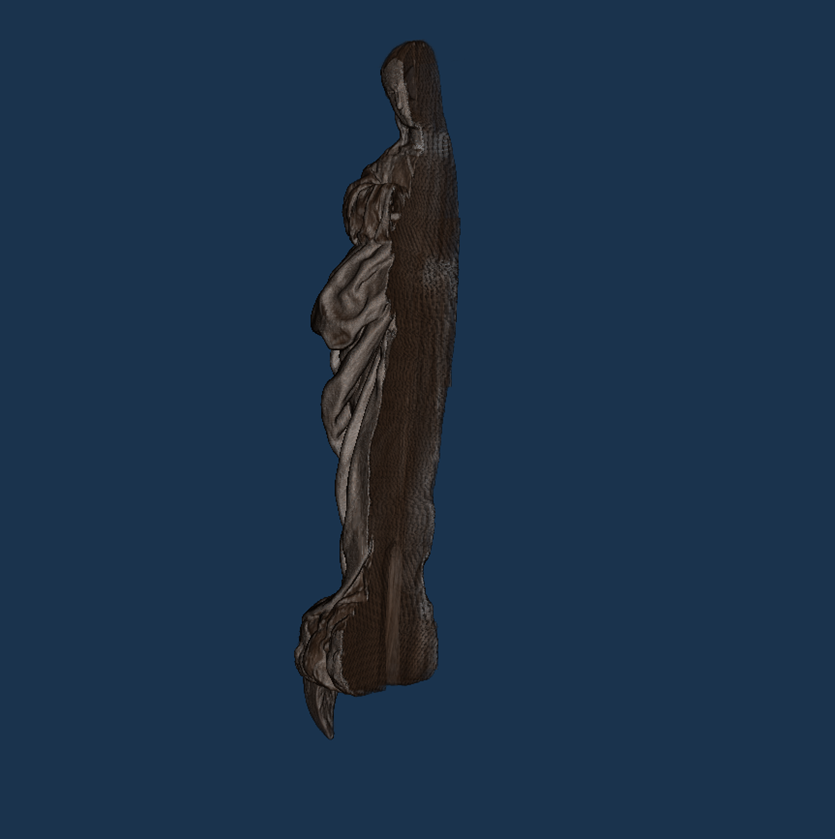
\includegraphics[width=6cm]{imagenes/resultados/segmentacion/inmaculada-concepcion/dcha-3d}
	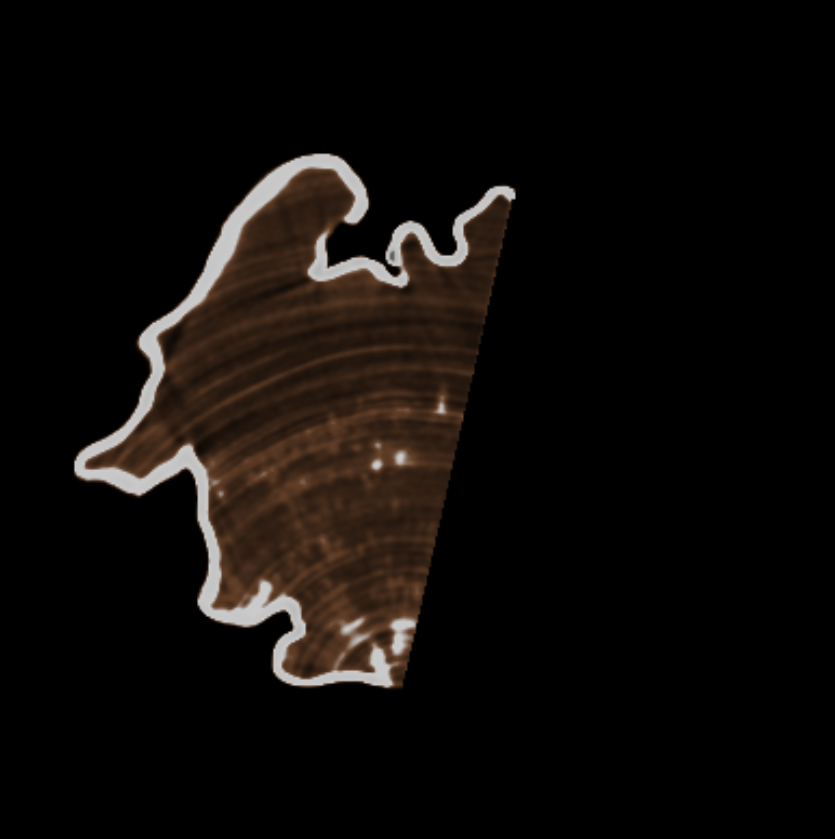
\includegraphics[width=6cm]{imagenes/resultados/segmentacion/inmaculada-concepcion/dcha-corte}
	\caption{Volumen con la pieza de la derecha y un corte donde se ve dónde ha cortado}
	\label{fig:resultados/segmentacion/inmaculada-concepcion/dcha}
\end{figure}

\begin{figure}[H]
	\centering
	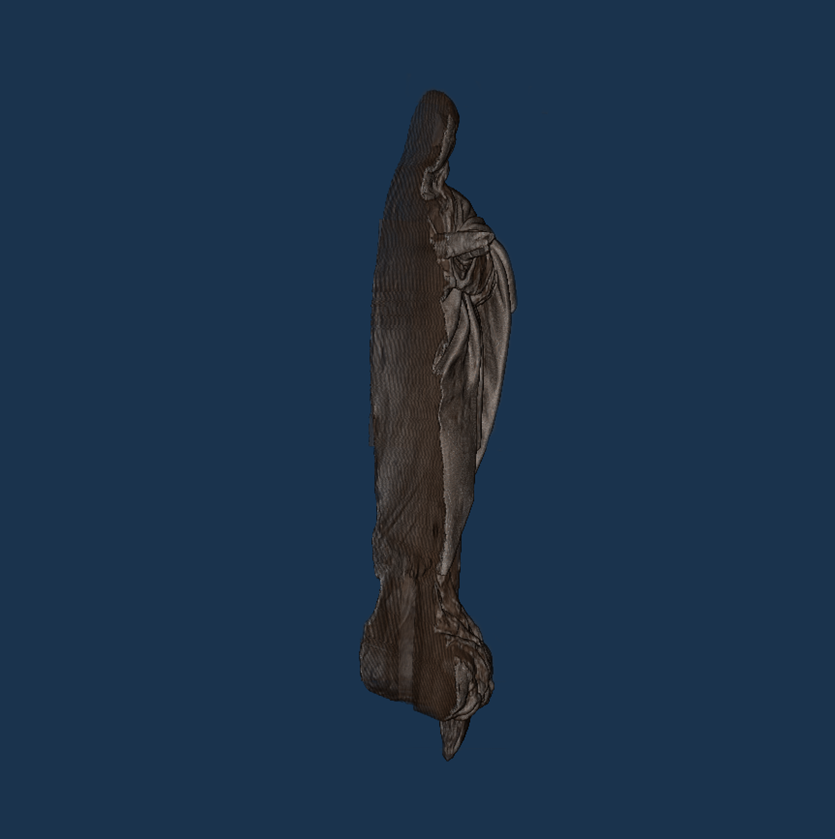
\includegraphics[width=6cm]{imagenes/resultados/segmentacion/inmaculada-concepcion/izda-3d}
	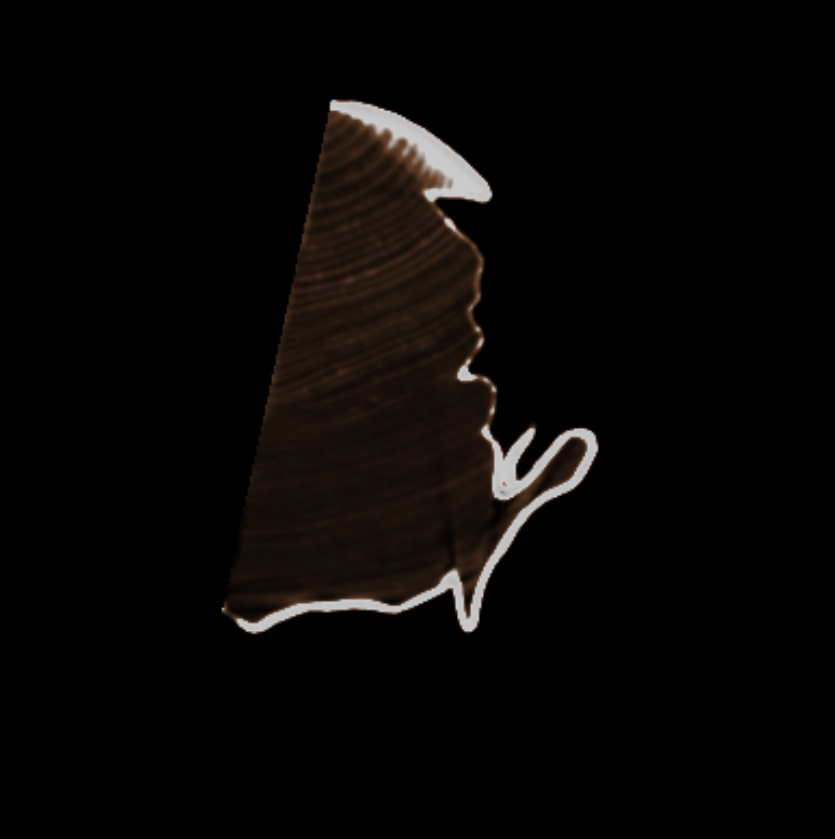
\includegraphics[width=6cm]{imagenes/resultados/segmentacion/inmaculada-concepcion/izda-corte}
	\caption{Volumen con la pieza de la izquierda y un corte donde se ve dónde ha cortado}
	\label{fig:resultados/segmentacion/inmaculada-concepcion/izda}
\end{figure}

\subsection{San Juan Evangelista}

En el San Juan Evangelista hay dos piezas principales en el embón una muy grande frontal y otra bastante más pequeña trasera. Esta pequeña no se puede ver por la zona de la cabeza y en la zona de la cintura hay un clavo que hace que no se diferencie muy bien la línea recta. Sin embargo, por la zona del pecho se puede encontrar una buena semilla donde se detecte la línea que corta ambas piezas de madera.

Se ha utilizado un corte por esta zona y se ha encontrado esta línea (Figura \ref{fig:resultados/segmentacion/inmaculada-concepcion/seleccion-linea}).

\begin{figure}[H]
	\centering
	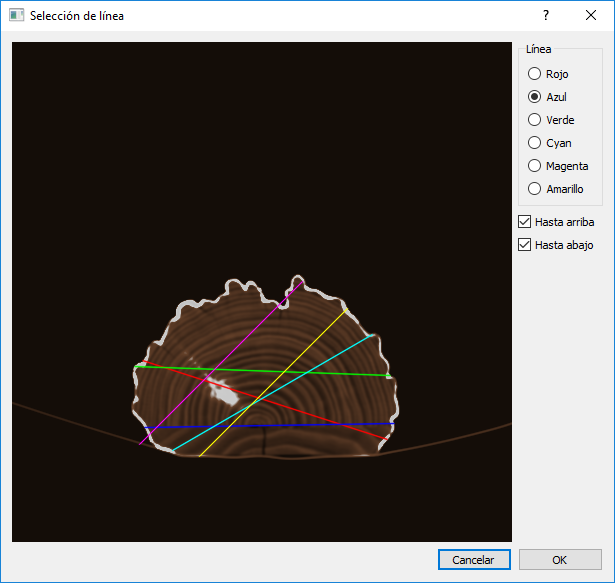
\includegraphics[width=12cm]{imagenes/resultados/segmentacion/san-juan-evangelista/seleccion-linea}
	\caption{Líneas encontradas en un corte a la altura de la cintura donde se ve la línea (azul) que separa las dos piezas del embón}
	\label{fig:resultados/segmentacion/san-juan-evangelista/seleccion-linea}
\end{figure}

Esta línea divide perfectamente en dos la figura obteniendo los resultados de a continuación (Figuras \ref{fig:resultados/segmentacion/san-juan-evangelista/frontal} y \ref{fig:resultados/segmentacion/san-juan-evangelista/trasero}).

\begin{figure}[H]
	\centering
	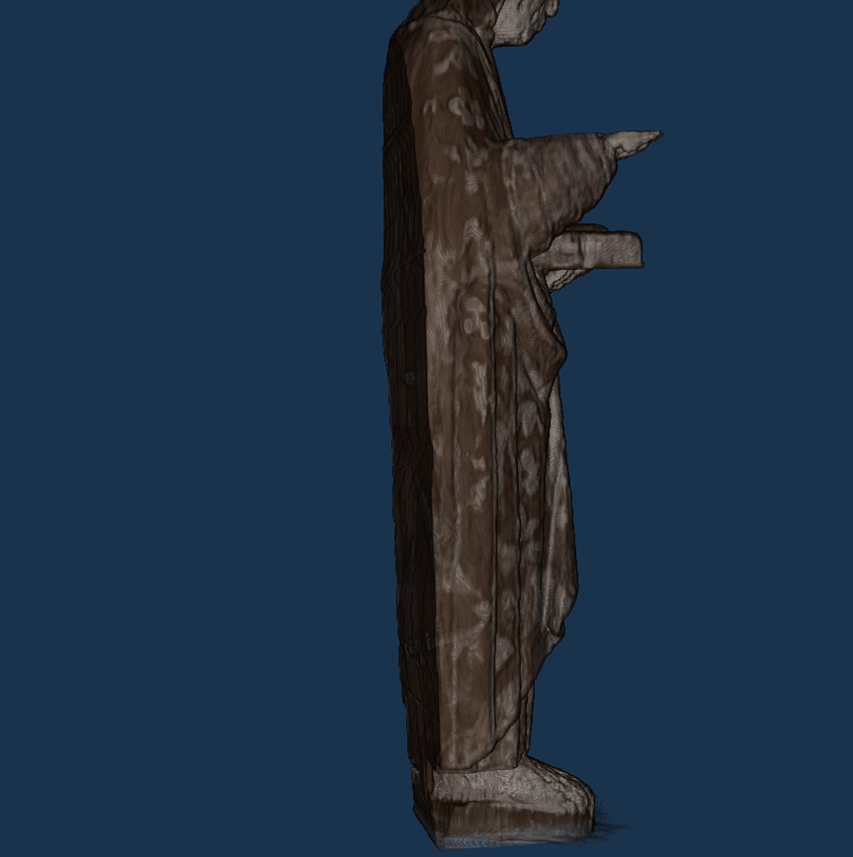
\includegraphics[width=6cm]{imagenes/resultados/segmentacion/san-juan-evangelista/frontal-3d}
	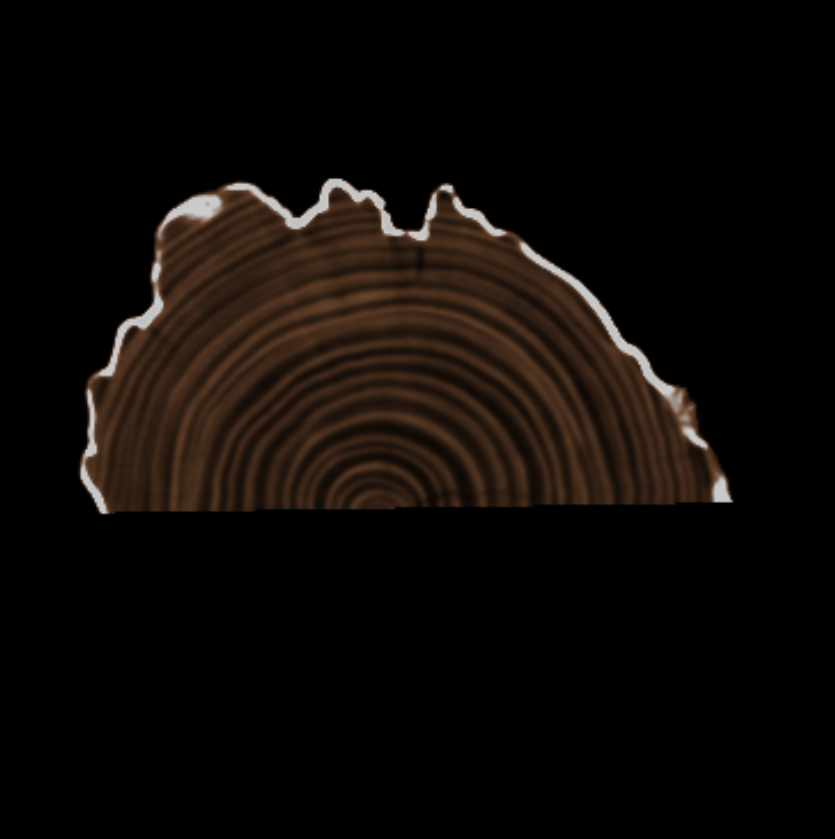
\includegraphics[width=6cm]{imagenes/resultados/segmentacion/san-juan-evangelista/frontal-corte}
	\caption{Volumen con la pieza frontal y un corte donde se ve dónde ha cortado}
	\label{fig:resultados/segmentacion/san-juan-evangelista/frontal}
\end{figure}

\begin{figure}[H]
	\centering
	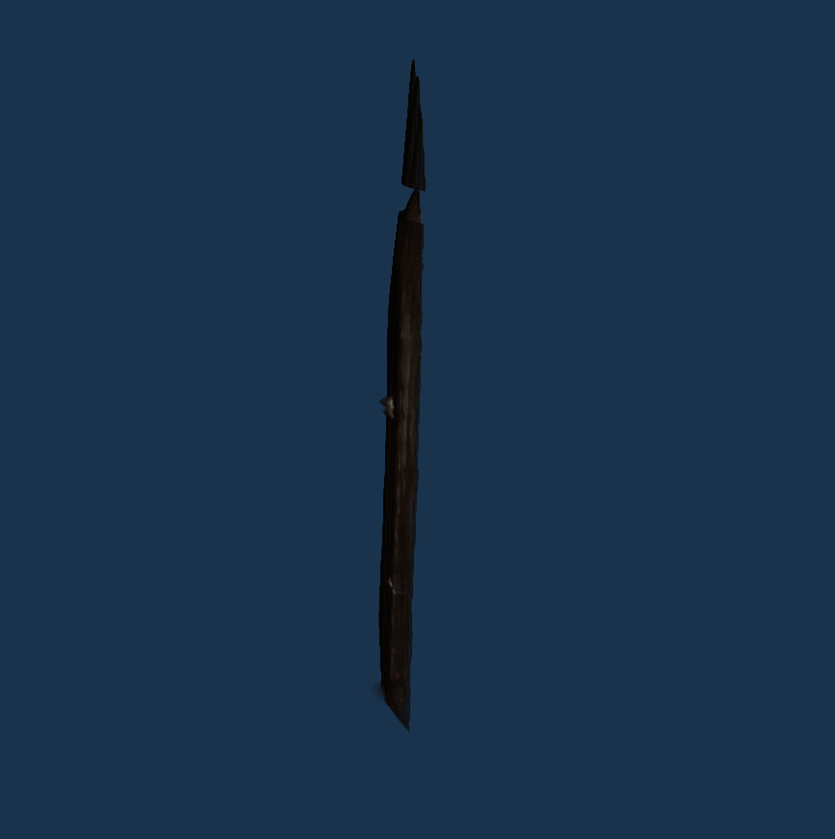
\includegraphics[width=6cm]{imagenes/resultados/segmentacion/san-juan-evangelista/trasero-3d}
	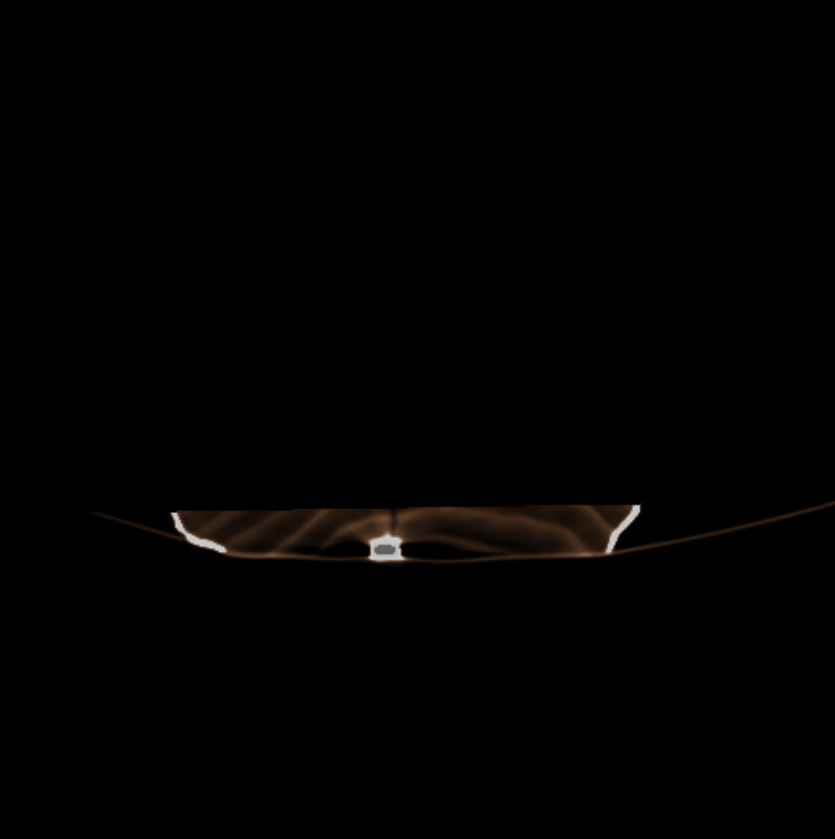
\includegraphics[width=6cm]{imagenes/resultados/segmentacion/san-juan-evangelista/trasero-corte}
	\caption{Volumen con la pieza trasera y un corte donde se ve dónde ha cortado}
	\label{fig:resultados/segmentacion/san-juan-evangelista/trasero}
\end{figure}